\chapter{NFC tehnologija}
NFC (Near Field Communication) je tehnologija dvosmjernog be�i?nog prijenosa podataka izme?u dva ure?aja u kratkom dometu. NFC je osmi�ljen da korisnicima pru�i siguran, brz i jednostavan pristup digitalnom sadr�aju, uparivanje ure?aja i beskontaktne transakcije.

Kao protokol posebno je zanimljiv industriji pametnih telefona jer su NFC moduli kompaktni i cjenovno pristupa?ni. Po�to ve?ina ljudi danas posjeduje pametni telefon, a samim tim i NFC ure?aj, razni proizvo?a?i mobilnih aplikacija implementiraju NFC povezivost u svoje aplikacije te time pro�iruju domenu funkcionalnosti koje nude svojim korisnicima. Primjer je mobilna aplikacija Foursquare \cite{foursquare} koja koriste?i NFC omogu?uje korisnicima da se prijave na razim mjestima interesa (POI point of interes) kao �to su restorani, hoteli, ulice... Kada korisnik pre?e pametnim telefonom do 10 cm iznad naljepnice aplikacija, koriste?i NFC senzor, skenira podatke o lokaciji POI-a koje u svojoj memoriji sadr�i NFC ure?aj. Logo Forsquare-a je prikazan na slici  ~\ref{fig:forsquare}.

\begin{figure}[!htbp]
	\begin{center}
 
\includegraphics[height=6cm,keepaspectratio=true]{nfc_forsquare}
 \caption{Logo aplikacije Forsquare}
 \label{fig:forsquare}
	\end{center}
\end{figure}

2004. godine je osnovano neprofitno dru�tvo NFC Forum \cite{nfc_forum} ?iji ?lanovi uklju?uju firme koje se bave razvojem i primjenom NFC-a u svim segmentima tehnologije. Cilj dru�tva je razvoj i standardizacija protokola i ure?aja koji ga koriste. NFC Forum su osnovale tvrtke Sony, Nokia i NPX Semiconductors, te dru�tvo danas broji preko 190 ?lanova. Neki od ?lanova su vode?e svjetske tehnolo�ke kompanije, kao npr. Apple, Google, Intel i Samsung. Na slici  ~\ref{fig:nfc} je prikazan logotip protokola.

\begin{figure}[!htbp]
	\begin{center}
 
\includegraphics[height=4cm,keepaspectratio=true]{nfc_logo}
 \caption{Logo NFC protokola}
 \label{fig:nfc}
	\end{center}
\end{figure}

\section{Arhitektura}

NFC komunikacija se sastoji od dva ure?aja koja u sebi sadr�e antene u obliku zavojnice:
\begin{itemize}
	\item Ure?aj koji inicira komunikaciju
	\item Ure?aj koji slu�a i ?eka da komunikacija bude inicirana
\end{itemize}

Komunikacija se vr�i preko magnetskog polja koje se stvara izme?u antena, sli?no kao kod elektri?nog transformatora. Komunikacija se vr�i na frekvenciji od 13.56 MHz i brzine je do 424 kbit/s. Maksimalna udaljenost izme?u dva ure?aja koja komuniciraju je 4 cm\textsuperscript{3}. Na slici ~\ref{fig:nfc_arhitektura} su prikazana oba ure?aja te magnetsko polje izme?u njih.


\begin{figure}[!htbp]
	\begin{center}
 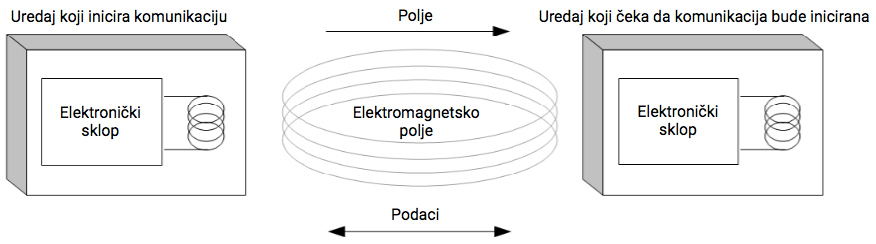
\includegraphics[height=4cm,keepaspectratio=true]{nfc_diagram}
 \caption{Komunikacija dva NFC ure?aja}
 \label{fig:nfc_arhitektura}
	\end{center}
\end{figure}

NFC ure?aji implementiraju dvije specifikacije i njihova funkcionalnost ovisi o tome po kojoj specifikaciji su izra?eni:

\begin{itemize}
	\item ISO/IEC 14443
	\begin{itemize}
		\item Definira memoriju NFC ure?aja
		\item Ure?aj je napravljen samo po ovoj specifikaciji je pasivni ure?aj i on ne mo�e inicirati komunikaciju (npr. naljepnica)
		
	\end{itemize}
	\item ISO/IEC 18092-3
	
	\begin{itemize}
		\item Definira elektromagnetsku komunikaciju (modulacije, kodiranje, inicijaliziaciju...)
		\item Ovi ure?aji implementiraju i ISO/IEC 14443 specifikaciju i oni su aktivni ure?aji
	\end{itemize}
\end{itemize}

Nadalje, ovisno o vrstama NFC ure?aja koji komuniciraju, komunikacija se dijeli na pasivnu i na aktivnu.


\subsection{Aktivna komunikacija}

Aktivna NFC komunikacija ozna?ava komunikaciju u dva smjera izme?u dva NFC ure?aja koji imaju vlastite izvore napajanja i napravljeni su po specifikaciji ISO/IEC 18000-3. Komunikacija se vr�i tako da ure?aj koji �eli poslati poruku aktivira svoje magnetsko polje preko kojega se poruka po�alje te ga deaktivira kada �eli primiti poruku. Ovakva komunikacija zahtjeva dodatnu logiku koja definira pravila komunikacije.

Aktivni NFC ure?aji se po arhitekturi dijele na:

\begin{itemize}
	\item NFC-A ure?aje
	\begin{itemize}
		\item Millerovo enkodiranje
		\item ASK modulacija 100%
		\item Brzina prijenosa 106 kb/s
	\end{itemize}

	\item NFC-B ure?aje
	\begin{itemize}
		\item Manchester enkodiranje
		\item ASK modulacija 10%
		\item Brzina prijenosa 106 kb/s
	\end{itemize}

	\item NFC-F (FeliCa) ure?aje
	\begin{itemize}
		\item Vrsta RFID protokola koja je jako sli?na NFC-u pa spada u istu kategoriju
		\item Razvijena je u Japanu gdje ima jako �iroku primjenu (najra�irenija je u kod prijevozni?kih karata)
		\item  Brzina prijenosa 212 kb/s
	\end{itemize}
\end{itemize}


\subsection{Pasivna komunikacija}

Pasivna komunikacija se vr�i izme?u aktivnog i pasivnog ure?aja, na na?in da aktivni ure?aj �alje signal nosioc kroz svoje elektromagnetsko polje. Ukoliko je pasivni ure?aj u dometu polje ?e inducirati napon u njegovoj zavojnici te ?e biti u stanju modulirati postoje?e polje, koriste?i ASK (amplitude-shift keying) modulaciju. To je znak aktivnom ure?aju da je komunikacija ostvarena. Nadalje, aktivni ure?aj pita pasivni koju vrstu komunikacije koristi (npr. komunikacija mo�e biti enkriptirana - koristi se kod pla?anja kreditnim karticama), te ovisno o odgovoru �alje odgovaraju?e zahtjeve za ?itanjem memorije, �to mu pasivni i pru�a, nakon �to ih uspje�no validira.



Tipovi pasivnih NFC ure?aja uklju?uju:

\begin{itemize}
	\item Tip 1
	\begin{itemize}
		\item Brisanje i ?itanje memorije
		\item Mogu se konfigurirati da se mogu samo ?itati
		\item Memorija: 96 B do 2kB
	\end{itemize}

	\item Tip 2
	\begin{itemize}
		\item Brisanje i ?itanje memorije
		\item Mogu se konfigurirati da se mogu samo ?itati
		\item Memorija: 48 B do 2kB
	\end{itemize}

	\item Tip 3
	\begin{itemize}
		\item Mogu ih ?itati samo NFC-F ure?aji
		\item Ili konfigurabilni (?itanje i pisanje) ili samo za ?itanje
		\item  Memorija varijabilna, teoretski mo�e biti do 1MB
	\end{itemize}

	\item Tip 4
	\begin{itemize}
		\item Ili konfigurabilni (?itanje i pisanje) ili samo za ?itanje
		\item Memorija do 32 KB
	\end{itemize}
\end{itemize}


\section{Primjena}

Razvoj dana�nje tehnologije pru�a ?ovje?anstvu sve opremljenije i prenosivije svakodnevne ure?aje. Samim time se je pojavila potreba za protokolom ?ija ?e primjena biti �to br�e i jednostavnije  prenjeti informacije sa ure?aja na ure?aj u kratkom dometu. Niska cijena, mogu?nost rada bez izvora energije i intinuitivnost kori�tenja (potrebno je samo prisloniti jedan NFC ure?aj o drugi) omogu?ava �iroku primjenu NFC-a, a neke njih uklju?uju:

\begin{itemize}
	\item Beskontaktno pla?anje kreditnim karticama ili pametnim telefonima
	\item Otklju?avanje ranih ure?aja (ra?unala, automobila, brava...)
	\item Razmjena vizitki
	\item ?itanje konfiguracije WiFi mre�e
	\item Vo?enje ?ita?a na internetsku poveznicu
	\item Ulaznice za razne doga?aje
\end{itemize}

Za potrebe ovog projekta kori�tene su NFC naljepnice kupljene preko internetske trgovine WhizTags \cite{whiztags}, prikazane na slici  ~\ref{fig:whiztags}.

\begin{figure}[!htbp]
	\begin{center}
 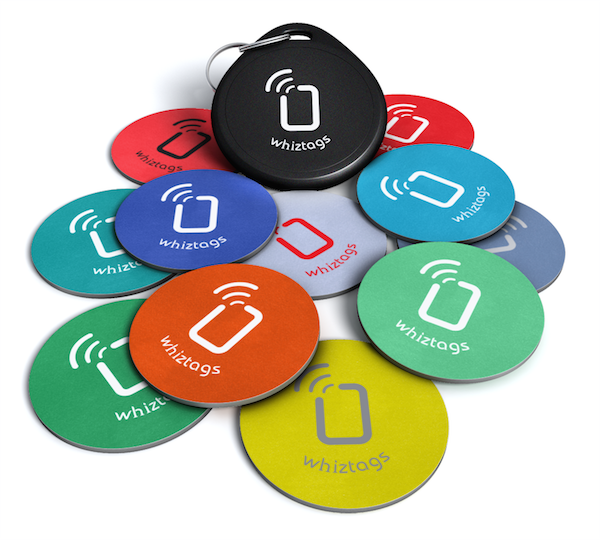
\includegraphics[height=8cm,keepaspectratio=true]{NTAG2161}
 \caption{Kori�tene NFC naljepnice}
 \label{fig:whiztags}
	\end{center}
\end{figure}

Specifikacija naljepnice:

\begin{itemize}
	\item NATG 216 NFC modul \cite{nat_modul}
	\item 888 B memorije
	\item Samoljepljivost
	\item Vodootpornost
\end{itemize}











